\chapter{Methodology}
\label{chap:methodology}
The methodology of this research will contain mainly 4 distinguishable parts. The first part covers research question 1. In this first section, the empirical study is clarified. The second section of this chapter covers research question 2, where the performance prediction of tools and strategies is enlightened. The third section will cover the ranking of these tools and strategies, covering research question 3. And in the fourth section, research question 4 is covered about the interpretability of the tools.

% The goal of the described methodology is to answer the main research question:
% \textit{How to choose a fitting error detection algorithm for a specific relational dataset?}

% RQ1
\section{Empirical study}
\label{sec:empiricalstudy}
% Both state of the art tools
% But also commonly used simpler tools
To substantiate further research questions with research data, a empirical study on error detection tools and different configurations is designed. To cover a broad range of configurations (strategies) of these tools, a range of permutations of configurations will be generated for each error detection tool and run on a wide range of datasets with different characteristics and errors. The source code of this framework can be found on GitHub\footnote{\url{\githubsource}}.
~\\Because the source languages of error detection tools differ, a high-level general purpose programming language suits to be used for the framework to connect all the different underlying tools. Together with the fact that it has well-supported libraries for relational data handling, Python\footnote{\url{\pythonsource}} was chosen as the main development language.


\subsection{Setup}
\label{subsec:setup}
First, the setup for the empirical study will be discussed. The basic setup is shown in figure \ref{fig:empiricalsetup}. For each tool in the study, a number of configurations is created, depending on the configurability of the tool. Each configuration in combination with that tool, will be tested on all the available datasets. So a single experiment exists of:
\begin{itemize}
    \item An error detection tool
    \item A tool specific configuration
    \item A target dataset
\end{itemize}

Each experiment will be pushed to the queue of experiments, allowing for retrieving a experiment session without having to rerun all the finished experiments. Incrementally, all the experiment results are pushed into the results database, allowing for the empirical study and further usage with performance prediction and tool ranking. 

\begin{figure}[h]
    \centering
    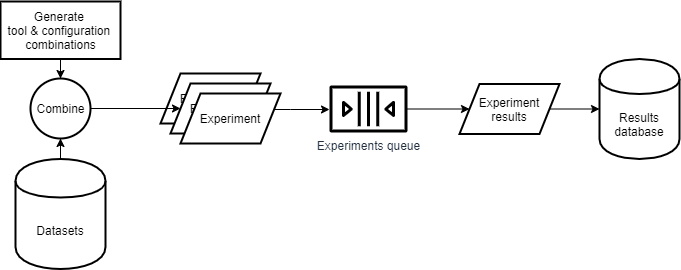
\includegraphics[width=\textwidth]{thesis/Figures/EmpiricalStudy.png}
    \caption{Setup of the empirical study}
    \label{fig:empiricalsetup}
\end{figure}

% Error detection API to do experiments
\subsection{Error detection framework}
First, a framework for running error detection tools was designed. The purpose of creating a single framework is to have homogeneous in and output for each selected error detection strategies, creating the possibility of running batches of experiments in a structured manner. 
The content and structure of the error detection framework is as follows:
\begin{itemize}[label=\ding{212}]
\item dataset
\item experiment
% \item helpers
%     \begin{itemize}[label=\ding{212}]
%         \item autofd
%         \item autoregex
%     \end{itemize}
\item profiler
\item tool
\item tools
    \begin{itemize}[label=\ding{212}]
        \item ...
        \item see section \ref{subsec:tools}
    \end{itemize}
\end{itemize}

\paragraph{dataset} contains the class for handling datasets for the experiments. It is based upon the work done by \cite{Mahdavi2019-zf} where each dirty dataset has a clean counterpart. Errors can be calculated both cell-wise as well as row-wise. Information about a dataset can be uploaded for later use and metrics like precision, recall and the F1-measure can be calculated from within this class.

\paragraph{experiment} contains the workflow depicted in figure \ref{fig:empiricalsetup}. Objects from this class can create the tool-configuration-dataset triples for the empirical study. Also, it contains the incremental queuing system for execution of experiments, which can be interrupted and resumed at will. Besides the workings shown in figure \ref{fig:empiricalsetup}, this part of the framework supports timeouts of the experiments, to shut down experiments whenever the preconfigured time limit is set. Lastly, it will upload the result metrics, configuration and runtime to a centralized database to further filter and analyze the results.

\paragraph{profiler} contains the elements to profile datasets and predict performance for different tools. This will be further discussed in section \ref{sec:performanceprediction}.

\paragraph{tool} contains the classes for creating error detection tool instances and the base class for tool. The tool creator dynamically finds added tools and is possible to return Tool instances for each error detection tool. Each error detection tool is adjusted to work in similar fashion. It contains an abstract method to run the code, expecting similar input and output for each tool. The tool base class has subprocess functionality to support the timeouts set by the experiment and to run non-Python code. The tool base class also cleans up left over subprocesses whenever timeouts are reached. 

\paragraph{tools} contains each error detection specific implementation of the Tool base class. Only the initialization and the \verb|run| method need to be implemented for each tool work, making it easy to extend this framework. Every tool is implemented in a different submodule. The implemented tools will be further discussed in subsection \ref{subsec:tools}. 



\subsection{Metrics}
\label{subsec:metrics}
To measure the performance of tools on test datasets, metrics of two types can be used. Cell-based and row-based metrics. The difference lies in what is taken as an entity while calculating scores.

\subsubsection{Cell-based metrics}
Cell-based metrics, are metrics that identify each cell in a dataset as a separate entity in the test set. Each cell will be counted as 1 positive or negative. 

\subsubsection{Row-based metrics}
Row-based metrics, are metrics that identify each row in a dataset as a separate entity in the test set. A row could contain multiple errors, but only the whole row is counted as 1 positive or negative.

\subsubsection{Scores}
In the case of error detection, instances are either erroneous (positive) or clean (negative). Because the ground truth of the datasets in section \ref{subsec:datasets} is known, the following metrics can be calculated directly after the execution of a tool.

\subsubsection{Examples}
\todo{Add visual example of scores \& row vs. cell based metrics}
\todo{Add visual example of different scores}


\subsection{Datasets}
\label{subsec:datasets}
The datasets selected contained different types of errors, to create a heterogeneous test set to compare the tools and configurations. Errors in a dataset are defined by the difference in the dirty dataset and clean dataset. So only the ground truth makes up an error. Errors can be seen as a transformation of the ground truth to some dirty value. These transformations could specify why the dirty version is wrong. Below are different "error types" that describe errors that have similar transformation between the dirty instance and the ground truth. Of course, there might be overlap in these transformation, as one type of transformation could have the same effect as another type, but these categorizations give an overview of the dataset quality one has to deal with.

\subsubsection{Error types}
The error types are derived from section \ref{subsec:errortypes}, with the addition of the "other errors", which contains errors that cannot be found or described by the default error type categories.

\begin{itemize}
    \item \textit{Outliers:} Values that are erroneous and do not fit in the (column) distribution of the dataset
    \item \textit{Pattern violations:} Values that are erroneous and do not fit in the common pattern of that column (i.e. 2k20 in stead of 2020). Also error values where content and pattern is correct, but with wrong spelling.
    \item \textit{Rule violations:} Also, empty values or missing value placeholders (N/A) that are replaced are supposed to be a real value. Inconsistent abbreviations or references to entities (like states, companies, universities, etc..).
    .\item \textit{Duplicates:} are different tuples, referring to the same real-world entity.
    \item \textit{Other error types:} examples of this type are values that are result of a classification (output) based on the other given columns, but the output is wrong. An error value where the content of the entity is changed, i.e. wrong categories, description or other matters that change the meaning of the underlying value.
\end{itemize}

% \begin{itemize}
%     \item \textit{Outliers:} Values that are erroneous and do not fit in the (column) distribution of the dataset
%     \item \textit{Pattern violations:} Values that are erroneous and do not fit in the common pattern of that column (i.e. 2k20 in stead of 2020)
%     \item \textit{Spelling errors:} Error values where content and pattern is correct, but with wrong spelling.
%     \item \textit{Inconsistent representations of entities:} Inconsistent abbreviations or references to entities (like states, companies, universities, etc..)
%     \item \textit{Missing values:} Empty values or missing value placeholders (N/A) that are replaced are supposed to be a real value
%     \item \textit{Wrong content:} An error value where the content of the entity is changed, i.e. wrong categories, description or other matters that change the meaning of the underlying value.
%     \item \textit{Classification errors:} Values that are result of a classification (output) based on the other given columns, but the output is wrong
% \end{itemize}

\subsubsection{Selected datasets}
A summary of the list of datasets used for the empirical study, performance estimation and ranking of error detection strategies can be found below (table \ref{tab:datasets}). The datasets were taken from published data from the following papers: 
\begin{itemize}
    \item ED2 by \cite{Neutatz2019-aw}
    \item Raha by \cite{Mahdavi2019-zf}
    \item REDS by \cite{Mahdavi2019-pk}
    \item CleanML by \cite{Li2019-ve}
\end{itemize}

\begin{table}[H]
\begin{adjustbox}{tabular=lllll,center}
Name        & Error types                                              \\ \hline
Beers       & Pattern violations \& Rule violations                    \\
Flights     & Pattern violations \& Rule violations                    \\
Hospital    & Pattern violations                                       \\
Rayyan      & Pattern violations \& Rule violations                    \\
Tax         & Pattern violations                                       \\
Toy         & Rule violations \& Other error types                     \\
Restaurants & Pattern violations \& Rule violations                    \\
Restaurant  & Pattern violations                                       \\
Movies      & Pattern violations, Rule violations \& Other error types \\
Movie       & Rule violations                                          \\
University  & Rule violations                                          \\
Uscensus    & Rule violations \& Other error types                     \\
KDD         & Outliers \& Other error types                            \\
EEG         & Outliers \& Other error types                            \\
Company     & Pattern violations                                      
\end{adjustbox}
\caption{Table with different datasets used and the common error types present in these datasets}
\label{tab:datasets}
\end{table}

\paragraph{Beers} 
List of different beers
Numeric ID's, foreign keys, Names in alphanumeric, City, state abbreviation, includes amount of ounces (float/int) \& percentage alcohol (float)
\\(Source: ED2, REDS, Raha)

\paragraph{Flights}
List of flight schedules
Contains id, source of data (abbrev/site?), flight number alphanumeric with dashes, scheduled and actual departure and arrival times in XX:XX a.m. format
\\(Source: ED2, REDS, Raha)

\paragraph{Hospital}
List of hospital experiments (Introduced errors)
index, ProviderNumber, HospitalName, Address1, Address2, Address3, City, State, ZipCode, CountyName, PhoneNumber, HospitalType, HospitalOwner, EmergencyService, Condition, MeasureCode, MeasureName, Score, Sample, Stateavg
\\(Source: REDS, Raha)

\paragraph{Rayyan}
List published articles
id, article\_title, article\_language, journal\_title, jounral\_abbreviation, journal\_issn, article\_jvolumn, article\_jissue, article\_jcreated\_at, article\_pagination, author\_list
\\(Source: REDS, Raha)

\paragraph{Tax}
List of american tax payers
f\_name, l\_name, gender, area\_code, phone, city, state, zip, marital\_status, has\_child, salary, rate, single\_exemp, married\_exemp, child\_exemp
\\(Source: REDS, Raha)

\paragraph{Toy}
Dummy set for testing purposes \& testing for generalizability
\\(Source: REDS, Raha)

\paragraph{Restaurants}
List of restaurants
id, name, streetAddress, city, state, zipCode, phone, website, priceRange, categories, ratingValue, neighborhood, payment-method, years-in-business, extra-phones, aka
\\(Source: ED2)

\paragraph{Restaurant}
Same idea as "Restaurants", but less columns
name, streetAddress, city, state, zipCode, telephone, website, priceRange, categories, ratingValue, neighborhood
\\(Source: CleanML)

\paragraph{Movies}
List of popular movies
Id, Name, Year, Release Date, Director, Creator, Actors, Cast, Language, Country, Duration, RatingValue, RatingCount, ReviewCount, Genre, Filming Locations, Description
\\(Source: ED2, REDS, Raha)

\paragraph{Movie}
Same as movies, but less and different columns
\\(Source: CleanML)

\paragraph{University}
This dataset contains 286 records about universities. Each record has 17 attributes including state, university name,
SAT scores, etc. The classification task is to predict whether the expenses are greater than 7,000 for each university. This dataset contains inconsistent representations for states and locations.
\\(Source: CleanML)

\paragraph{Uscensus}
This dataset contains 32,561 US Census records
for adults. Each record has 14 attributes including age, education, sex, etc. The classification goal is to predict whether the adult earns more than \$50,000. This dataset contains missing values.
\\(Source: CleanML)

\paragraph{KDD}
This dataset contains 131,329 records about projects and
donations from DonorsChoose.org. Each record has 100 attributes.
The classification task is to predict whether a project is “exciting”.
This dataset has a class imbalance problem. There are 11% records
in the minority class. This dataset contains missing values and numerical outliers. We inject mislabels into this dataset by randomly
flip labels.
\\(Source: CleanML)

\paragraph{EEG}
This is a dataset of 14,980 EEG recordings. Each record
has 14 EEG attributes. The classification task is to predict whether
the eye-state is closed or open. This dataset contains numerical outliers. We inject mislabels into this dataset by randomly flip labels
\\(Source: CleanML)

\paragraph{Company}
List of companies
Some sort of capture date, id, long \& lat, sentiment about it, Company Name, Country, City, State (non abbreviated)
\\(Source: CleanML)

\subsection{Tools}
\label{subsec:tools}
In this subsection, the tools used in the case study will be discussed. The extensive summary of the workings of the tools can be found in section \ref{chap:background}.

\subsubsection{Raha \cite{Mahdavi2019-zf}}
A human-guided but configuration-free error detection system. It selects different preconfigured strategies automatically, based on previously cleaned datasets. Then, it incorporates the \textbf{outputs from various error detection strategies} as a feature vector for the error detection task. Using these feature vectors, it creates clusters of which samples will be labeled in order to reduce user involvement.

\subsubsection{Forbidden Itemsets \cite{Rammelaere2019-ea}}
Applies \textbf{constraint-like method} to detect and repair invalid entries in a dataset. The proposed so-called forbidden itemsets capture unlikely value co-occurrences, similar to denial constraints.

\subsubsection{FAHES \cite{Qahtan2018-te}}
A disguised missing values detector. Whereas most missing value detector focus only on NULL or empty values, this tool takes a different approach. They \textbf{categorize detectable disguised missing values} into five different cases: 1. Out of range data values 2. Outliers 3. String with repeated characters or characters that are next to each other on the used keyboard 4. Values with non-conforming data types 5. Valid values that are randomly distributed within the range of the data and used frequently in the data set.

\subsubsection{HoloClean \cite{Rekatsinas2017-iw}}
HoloClean, a data cleaning system that relies on \textbf{statistical learning and inference} to unify a range of data repairing methods. Contributions in this tool include: 1. a compiler that generates a probabilistic model which unifies different signals for repairing a dataset 2. an algorithm that uses Bayesian analysis to prune the domain of the random variables corresponding to noisy cells in the input dataset to systematically tradeoff the scalability and quality of repairs 3. an approximation scheme that relaxes hard integrity constraints to priors over independent random variables.

\subsubsection{dBoost \cite{Pit--Claudel2016-dj}}
Outlier Detection in Heterogeneous Datasets using Automatic Tuple Expansion. It uses \textbf{expansion of data tuples using knowledge about the schema and field types}. For example, a timestamp 1424866716 could be expanded into year 2015, Wednesday, etc.. Then outliers are detected based upon these schemas.

\subsubsection{KATARA \cite{Chu2015-fs}}
A \textbf{knowledge base} and crowd powered data cleaning system that, given a table, a knowledge base, and a crowd, interprets table semantics to align it with the knowledge base. Identifies correct and incorrect data, and generates top-k possible repairs for incorrect data.

\subsubsection{ActiveClean \cite{Krishnan2016-rg}}

% \subsubsection{Adapted tools}
% \label{subsubsec:adaptedtools}

\subsection{Execution \& Analysis}
To answer research question 1; \textit{What is the current state of the art and what is the performance of these tools?}; The different parts from the sections above will be combined. The tools in section \ref{subsec:tools} will be run in selected configurations (tool specific) on all the datasets from section \ref{subsec:datasets}. The main metrics that will be kept are cell-wise precsion, recall and F1-score. In a single experiment, a timeout limit is set to filter out tool configuration that do not satisfy runtime needs. The results will be aggregated into showing the best results for a single tool (regardless of its configuration) and the target dataset. This will be shown in a table where the rows represent a single dataset, and each column represents a tool. Such a table will allow quick comparison to see which of the tools performs best for which dataset.
\\Additionaly, these tables can be repeatedly be created with filters (such as no human interaction) or grouping the best scores per tool and dataset based on the selected metrics (i.e. best precision or best F1-score).
% RQ2
\newpage
\section{Performance prediction}
\label{sec:performanceprediction}
The next step is to answer the second research question: \textit{Is it possible to create an extensive data profile to estimate performance on unseen datasets?}; 

This can be answered by using the results given by the empirical study (\autoref{sec:empiricalstudy}) for predicting performance on unseen new datasets. The goal of performance prediction, is to estimate the performance scores of an error detection strategy, on a specific dataset, without having to run the strategy beforehand or having the clean dataset at hand. The data/work flow of this process is shown in \autoref{fig:method_estimation}.
When estimators are capable of estimating the performance scores, one could use this estimation to choose an error detection strategy. This contributes to the main research question of choosing a fitting error detection algorithm for a specific relational dataset.

To make predictions on the performance scores, information about the dataset is extracted beforehand, called a dataset profile. This profile contains high-level information that is of low cost computationally. This high-level information will most presumably give an idea on how to fix the errors inside the dataset, which could be input to predict the performance score a specific error detection strategy will get on that particular dataset. An estimator then is trained for each error detection strategy, with the all the data profiles. The main notion is that error detection strategies assumably have comparable performance scores on similar datasets in terms of these high-level information profiles. 

\begin{figure}[h]
	\centering
	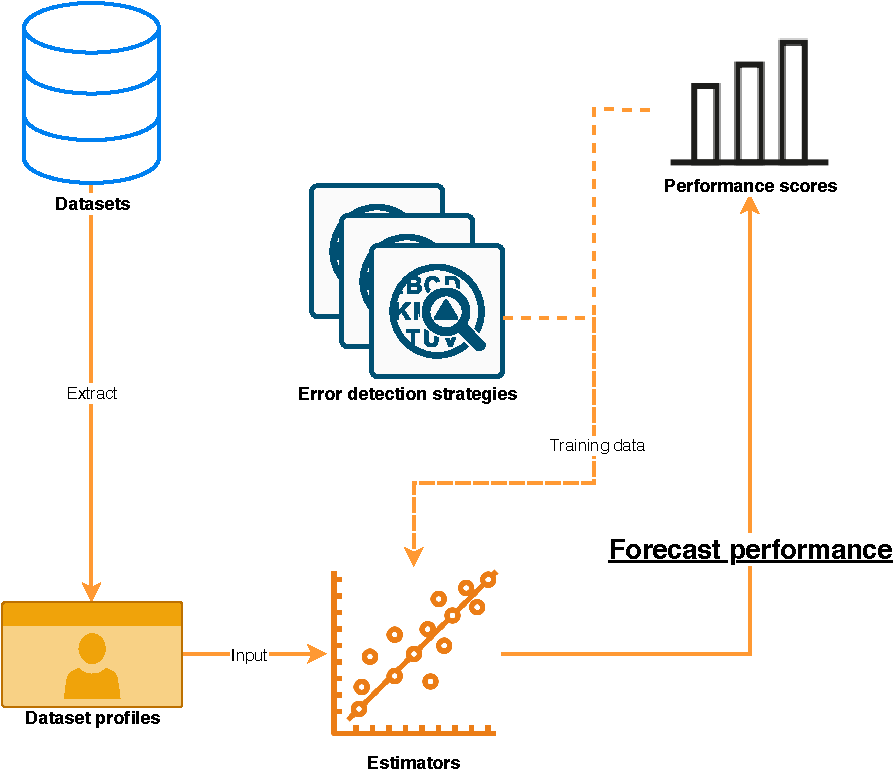
\includegraphics[width=0.9\textwidth]{thesis/Figures/Method/PerformanceEstimation-Profiler.pdf}
	\caption{Performance scores estimation}
	\label{fig:method_estimation}
\end{figure}

\newpage
\paragraph{Analogy} One can think of this like going into a car garage with a broken car. The employee of the garage will take a quick look at the outside of the car, at the brand of the car and will ask you some questions about the problems you have. This small \textit{\textbf{assessment}} could give an idea on what fixing strategy will most probably work best to fix the car. In his mind, the employee will have a list of strategies to fix a car (replace tyres, oil change, etc..) and will \textbf{\textit{estimate the possible outcomes}} (or performance) of those strategies (speed of fixing, longetivity, cost, etc..), based on the performance of these strategies on previous cars with a similar assessment. Although in the execution, the results might differ from what the employee had in mind. The estimation might not give the exact performance outcome.

This is the same with the prediction of the performance scores of error detection strategies as depicted in \autoref{fig:method_estimation}. An estimator, in this case a regression model, will look at a dataset and do the small assessment (\textbf{\textit{dataset profile}}), like looking at the car. From this small assessment, the estimator will try to \textbf{\textit{estimate the performance scores}} for each of the error detection strategies in mind based on previous datasets and the performance on those datasets, like the car garage employee guessed the outcome of replacing the tyres based on experience with previous cars. However, will be a difference between the real outcome of that strategy (experimental results from \autoref{sec:empiricalstudy}) and the estimations of the performance scores. 

This idea was proposed by \cite{Mahdavi2019-pk}. This paper proposes the idea of a 'dirtiness profile'. The idea is that error detection tools would have similar performance on similar datasets. Regression models would be trained and tested on characteristics of the dataset, also called 'dirtiness profile' (input) and F1-scores (output). The following section will be a modification of the research by \cite{Mahdavi2019-pk}. 
The goal will be to estimate performance and predict values as close to the real performance scores as possible, which can be measured with the mean squared error.
The train and test in and outputs are retrieved from the empirical study (\autoref{sec:empiricalstudy}). One main difference is that this research will solely focus on automated prediction, where no rules or patterns from the ground truth are taken and no user defined configurations need to be created in order to perform the predictions. Besides, multiple new input features will be introduced to see if the performance can be increased. Lastly, instead of directly estimating the F1-score, as done by \cite{Mahdavi2019-pk}, estimators will be trained on both the recall and precision scores. The F1-score can the be calculated using both estimated scores.
A regression model is trained for every strategy (error tool and specific configuration, see \autoref{fig:eachstrategy}). 

\begin{figure}[h]
	\centering
	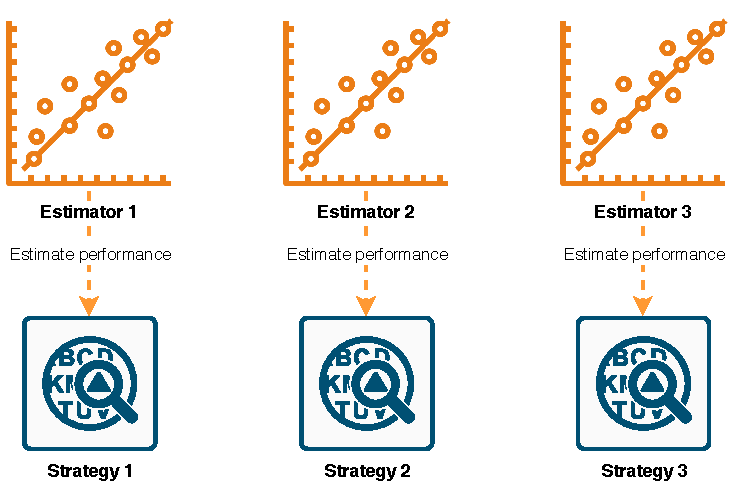
\includegraphics[width=0.8\textwidth]{thesis/Figures/Method/PerformanceEstimation-OnlyEstimate.pdf}
	\caption{Each strategy will result in a separate estimator}
	\label{fig:eachstrategy}
\end{figure}

\subsection{Data profiles}
\label{subsec:dataprofiles}
To answer the first part of the second research question: \textit{Is  it  possible  to  \textbf{create an extensive data profile} to estimate performance on unseen datasets?}, this section will discuss the methodology of creating such a data profile for a dataset.
The data profiles are created using only top-level features, without having any previous knowledge about the datasets. In this research, the focus lies only on features that are extractable without knowing the ground truth, only the dirty dataset. The basic set of features used is a subset of the proposed features from \cite{Mahdavi2019-pk}. However, all features where some information about the ground truth was necessary (rules, patterns or other heuristics found in the clean dataset), were left out. The extracted features extracted from each column. Then, aggregates of these column-wise extracted features are aggregated using the mean, variance, min and max to get a representation of feature distributions for each column in a dataset, with homogeneous output in size for training the regression models later on. These aggregated features representing the dataset profiles are the input values for the estimators. 

\begin{table}[H]
\centering
\begin{adjustbox}{center}
	\begin{tabular}{lll}
		Feature                   & Type       & Description \\ \hline
		characters\_unique        & characters & The number of unique characters \\
		characters\_alphabet      & characters & The number of only alphabetical characters \\
		characters\_numeric       & characters & The number of only numerical characters \\
		characters\_punctuation   & characters & The number of punctuation characters \\
		characters\_miscellaneous & characters & The number of characters not included in the categories above \\
		words\_unique             & words      & The number of unique words \\
		words\_alphabet           & words      & The number of fully alphabetical words \\
		words\_numeric            & words      & The number of fully numerical words (decimals included) \\
		words\_punctuation        & words      & The number of characters used solely as punctuation \\
		words\_miscellaneous      & words      & The number of words not included in the categories above  \\
		words\_length             & words      & The average word length \\
		cells\_unique             & cells      & The number of unique cells \\
		cells\_alphabet           & cells      & The number of completely alphabetical cells \\
		cells\_numeric            & cells      & The number of fully numerical cells (decimals included) \\
		cells\_punctuation        & cells      & The number of cells with only punctuation characters \\
		cells\_miscellaneous      & cells      & The number of cells not included in the categories above\\
		cells\_length             & cells      & The total length of cells combined \\
		cells\_null               & cells      &  The number of empty cells 
	\end{tabular}
	\end{adjustbox}
	\caption{All column-wise extracted features for the dataset profiles}
	\label{tab:profilefeatures}
\end{table}

\subsection{Experimental setup}
%%% Leave-one-out training
% Real performance dataframe
% Estimation performance dataframe
% Calculate errors
To answer the other part of the second research question: \textit{Is it  \textbf{possible} to create an extensive data profile \textbf{to estimate performance} on unseen datasets?}, this section will describe the proposed experiment to test the estimation capabilities of possible estimators. 
To discover whether the discussed data profiles are useful in estimating the performance of error detection tools, the setup from \autoref{sec:empiricalstudy} is updated. \autoref{fig:method_estimation} shows the flow of estimating the performance scores of the run error detection tools on the datasets. The goal of this workflow is to estimate the performance scores of error detection strategies on unseen datasets.

The estimators will be created as scikit-learn (\cite{Pedregosa2011-su}) pipelines. Not only does this allow interchangeable regression models, but also configurable data preparation. The different configurable parts all have certain assumptions. A combinination of all possible settings will be created and tested, in order to find the best configuration possible.

To evaluate the estimators and find the best configuration for the estimators, an experiment has to be conducted to evaluate the prediction potential of these estimators.
In reality, the estimators will be trained on all available training datasets and will be used to estimate performance scores on unseen datasets. However, with unseen datasets, only the dirty dataset is available, not the clean dataset. This means that it is not possible evaluate the prediction capabilities of these estimators in a straight-forward way.
\textbf{Leave-one-out cross validation} is a method to simulate the behaviour of training on as many training datasets as possible, while still being able to evaluate the results afterwards, by leaving only one dataset out of that training set at the time. \autoref{tab:leave-one-out} shows such an example for leave-one-out training with 4 datasets available. In each iteration, a single dataset is left out of the training set, simulating the performance prediction for the left out dataset. This will result in a performance score prediction $\hat{y}(s_i, d_j)$ for a certain strategy $s_i$ and dataset $d_j$. 

 \begin{table}[H]
\centering
\begin{tabular}{|l|l|l|l|l|l|}
\cline{1-4} \cline{6-6}
\textbf{$d_1$} & \textbf{$d_2$} & \textbf{$d_3$} & \textbf{$d_4$} &                 & \textbf{Output} \\ \cline{1-4} \cline{6-6} 
\textit{Estimate}          & Train         & Train         & Train         & $\rightarrow$ & $y(s_i, d_1)$      \\ \cline{1-4} \cline{6-6} 
Train         & \textit{Estimate}          & Train         & Train         & $\rightarrow$ & $y(s_i, d_2)$      \\ \cline{1-4} \cline{6-6} 
Test          & Train         & \textit{Estimate}          & Train         & $\rightarrow$ & $y(s_i, d_3)$     \\ \cline{1-4} \cline{6-6} 
Test          & Train         & Train         & \textit{Estimate}          & $\rightarrow$ & $y(s_i, d_4)$      \\ \cline{1-4} \cline{6-6} 
\end{tabular}
\caption{Leave one out training example for a strategy $s_i$ and datasets $d_{1-4}$}
\label{tab:leave-one-out}
\end{table}

For each dataset $d$ from $D$ datasets and error detection strategy $s$ from all strategies $S$, the leave-one-out evaluation as described above and in \autoref{tab:leave-one-out} will be executed. This will leave a $m \times n$ matrix of estimated performance scores as shown in \autoref{tab:estimatedscores}, representing a $m$ strategies and the $n$ available datasets.
For comparison, the real scores that are obtained from the empirical study from \autoref{sec:empiricalstudy} are shown in the same format in \autoref{tab:realscores}.

 \begin{table}[h]
	\centering
	\addtolength{\leftskip} {-2cm}
	\addtolength{\rightskip}{-2cm}
	\captionsetup[subtable]{position = below}
	\captionsetup[table]{position=top}
	\caption{$m \times n$ (strategies $\times$ datasets) matrix of scores}
		\begin{subtable}{0.5\linewidth}
		\centering
		\begin{tabular}{|l|l|l|l|l|}
			\hline
			               & \textbf{$d_1$}      & \textbf{$d_2$}      & \textbf{...} & \textbf{$d_n$}      \\ \hline
			\textbf{$s_1$} & $\hat{y}(s_1, d_1)$ & $\hat{y}(s_1, d_2)$ & ...          & $\hat{y}(s_1, d_n)$ \\ \hline
			\textbf{$s_2$} & $\hat{y}(s_2, d_1)$ & $\hat{y}(s_2, d_2)$ & ...          & $\hat{y}(s_2, d_n)$ \\ \hline
			\textbf{...}   & ...                 & ...                 & ...          & ...                 \\ \hline
			\textbf{$s_m$} & $\hat{y}(s_m, d_1)$ & $\hat{y}(s_m, d_2)$ & ...          & $\hat{y}(s_m, d_n)$ \\ \hline
		\end{tabular}
		\caption{Estimated performance scores}
		\label{tab:estimatedscores}
	\end{subtable}
	\hspace*{4em}
	\begin{subtable}{0.5\linewidth}
		\centering
		\begin{tabular}{|l|l|l|l|l|}
			\hline
			               & \textbf{$d_1$} & \textbf{$d_2$} & \textbf{...} & \textbf{$d_n$} \\ \hline
			\textbf{$s_1$} & $y(s_1, d_1)$  & $y(s_1, d_2)$  & ...          & $y(s_1, d_n)$  \\ \hline
			\textbf{$s_2$} & $y(s_2, d_1)$  & $y(s_2, d_2)$  & ...          & $y(s_2, d_n)$  \\ \hline
			\textbf{...}   & ...            & ...            & ...          & ...            \\ \hline
			\textbf{$s_m$} & $y(s_m, d_1)$  & $y(s_m, d_2)$  & ...          & $y(s_m, d_n)$  \\ \hline
		\end{tabular}
		\caption{Real performance scores}
		\label{tab:realscores}
	\end{subtable}%
\end{table}
       

To assess the estimated performance scores as shown in \autoref{tab:estimatedscores}, the scores will be compared element-wise with the real performance scores shown in \autoref{tab:realscores}. To do so, the difference between the estimation of the score and the score itself will be calculated. This is the \textbf{estimation error}. 
The real score is denoted as $y$, which is a performance score result of the empirical study, for example precision, recall or f1-score. The estimated score is denoted as $\hat{y}$. The error for a single score, for a specific error detection strategy and dataset is the following:

\begin{equation}
	e(s, d) = \hat{y}(s, d) - y(s, d)
\end{equation}

To quantify the ability of an estimator pipeline to estimate the real performance scores of error detection strategies, the mean square error for all the (strategy, dataset) tuples is taken. 

\begin{equation}
	MSE = \frac{1}{|D||S|} \sum_{d \in D} \sum_{s \in S} e(s, d)^2
\end{equation}

This mean square error will give a method of comparison between different estimator configurations. For the best estimator configuration, the estimation error distribution will be shown to find how the estimator generally performs, for example by comparing the number of over- and under-estimations.

\subsection{Estimator selection}
\label{subsec:estimatorselection}
% Regression model selection
Now that a score for comparing estimators has been covered, the range of estimator configurations will be discussed.
The estimator pipeline consists of 4 possible parts:
\begin{enumerate}
	\item Feature normalization
	\item Feature selection
	\item Principle component analysis
	\item Regression model
\end{enumerate}

Each part of the pipeline is configurable. The first three parts can be left out, leaving only a regression model with the normal dataset profile as input. 

\subsubsection{Feature normalization or standardization}
The three chosen possibilities for feature normalization are:
\begin{itemize}
	\item None: No normalization or scaling is applied.
	\item StandardScaler (\verb|sklearn.preprocessing.StandardScaler|): Standardize features by removing the mean and scaling to unit variance. The scaler will be trained on the training sample so to that after the training, each feature can be scaled using the distributions of the training set.
	\item Normalizer (\verb|sklearn.preprocessing.Normalizer|): Normalize samples individually to unit norm. Each sample (i.e. each row of the data matrix) with at least one non zero component is rescaled independently of other samples so that its norm equals one. It is executed with a default $l_2$-norm
\end{itemize}

\subsubsection{Feature selection}
For feature selection, different trainable configurations are possible to optimize the amount of input dimensions for the later parts of the pipeline. Research has shown that using too many input features for machine learning will decrease performance (\cite{Trunk1979-sq}). To circumvent the curse of dimensionality, feature selection methods can be put in the machine learning pipeline to learn which features to use as well. 

\begin{itemize}
	\item None: No dimensionality reduction is applied in the pipeline.
	\item Variance Threshold (\verb|sklearn.feature_selection.VarianceThreshold|): This removes all features that in have a variance below a certain threshold in the training dataset. The threshold has to be set to some value.
	\item Select From Model (\verb|sklearn.feature_selection.SelectFromModel|): It selects the features based upon the importance weights of the trained regressor. On default, all features that have a weight above the mean of all feature weights are selected.
	\item Select K Best (\verb|sklearn.feature_selection.SelectKBest|): This method selects the K best features according to a specified score. In this case, the \\\verb|sklearn.feature_selection.f_regression| method is used, where the correlation between the target values and each separate (univariate) feature is calculated.
\end{itemize}

Besides feature selection that will be learned from the input features, are trainable and present in the machine learning pipeline, feature selection can be done in retrospect, which will be discussed in \autoref{subsec:featureselection}.

\subsubsection{Principle component analysis}
Principle component analysis is a dimensionality reduction method invented over a century ago (\cite{Pearson1901-de}), but still has a strong use case in machine learning today. As said in the previous section, too many input features will lead to worse performance with the small amount of input samples to train. A linear PCA will reduce the whole feature space to N number of components holding the most variance for all the input points. To transform and capture non-linear relations, also Kernel PCA will be used. This will be useful, as most regressorion models will not be capable of distinguishing between non-linear relations.

\begin{itemize}
	\item None: No dimensionality reduction using PCA will be done.
	\item PCA (\verb|sklearn.decomposition.PCA|): Linear dimensionality reduction using Singular Value Decomposition of the data to project it to a lower dimensional space. Highly sensitive to scaling of the features (recommended to scale beforehand).
	\item Kernel PCA (\verb|sklearn.decomposition.KernelPCA|): Allows for non-linear dimensionality reudction through using specified kernels. A RBF (radial basis function) kernel is commonly used for projecting non-linear relation onto a linear separable projection.
\end{itemize}

\subsubsection{Regression model}
As the final step in the pipeline, a regression model is present. It takes in the input features from the last step in the pipeline, depending on which normalization, feature selcetion and/or principle component analysis methods are chosen. The regression model will take the transformed data profile inputs from all the training datasets and tries to estimate the selected real scores. This score always will be between 0 and 1, inclusive. So at the end of each estimator, a limiter will be put into place to not have any impossible scores. The possible regression models are stated below. All models have certain assumptions that the workings build upon. 

\begin{itemize}
	\item Linear Regression (\verb|sklearn.linear_model.LinearRegression|): This regression model fits a linear model that minimizes the sum of errors between the observed estimation and real observations. This method can be sensitive to outliers, due to its reliance on the square of errors.
	\item K-nearest Neighbors Regression (\verb|sklearn.neighbors.KNeighborsRegressor|): The output is estimated by comparing it to the nearest neighbors in the training samples. The K nearest points are weighted equally and the training scores will be combined as estimation.
	\item Ridge Regression (\verb|sklearn.linear_model.Ridge|): This model solves a regression model where the loss function is the linear least squares function and regularization is given by the $l_2$-norm
	\item Bayesian Ridge Regression (\verb|sklearn.linear_model.BayesianRidge|): This model can be used for estimating the regularization parameters as well, the regularization parameter is not set in a hard sense but tuned to the data at hand. It then estimates the ridge regression model.
	\item Decision Tree Regression (\verb|sklearn.tree.DecisionTreeRegressor|): This is a regression model that outputs different discrete output levels based on an outcome of a decision tree, comparing individual features to certain learned values.
	\item Support Vector Regression (\verb|sklearn.svm.SVR|): A support vector machine based regression model. Like normal Support Vector Classification, the regression model depends only on a subset of the training data, making it more robust against outliers.
	\item Gradient Boosting Regression (\verb|sklearn.ensemble.GradientBoostingRegressor|): Produces a predictive model from an ensemble of weak predictive models. In each stage a regression tree is fit on the negative gradient of the least squares regression loss.
	\item AdaBoost Regression (\verb|sklearn.ensemble.AdaBoostRegressor|): A meta-estimator that trains multiple regression models (default \verb|DecisionTreeRegressor|) and consequently adjust weights of input samples depending on the error of the previous estimator.
	\item Multi-layer Perceptron Regression (\verb|sklearn.neural_network.MLPRegressor|): A neural network based regression model. Capable of capturing non-linear relations, however that would require multiple layers, which will on its turn require more training samples. 
\end{itemize}

\subsection{Combination of estimators}
% Separate precision & recall estimator
% Combined values
Now that all the components for the estimator have been described, one can try to create ensemble estimators. In the study of \cite{Mahdavi2019-pk}, the F1-score was directly estimated. Knowing that this metric is directly build from both the precision and recall, it intuitively makes sense to first create estimators for the precision and recall (separate 2 estimator configurations), and use the output of these two configuration in combination to estimate the F1-score. Therefore, besides only calculating the MSE for a F1-score estimator, it will be compared to the MSE of the ensemble F1-score estimator.

\subsection{Evaluation}
\label{subsec:evaluation_performanceprediction}
To evaluate the experiment results as discussed above, the results will be both qualitatively and quantitatively analyzed to find an answer the research question: \textit{Is it possible to create an extensive data profile to estimate performance on unseen datasets?};

\paragraph{Qualitative} First, the best estimator configuration will be chosen according the lowest mean squared error of the estimations of real performance scores. This chosen estimator configuration will be qualitatively be judged on the distribution of estimation errors. In order to deem the estimation of performance successful, the error distribution should be heavily centered around 0, indicating that most estimations are close to perfect. Also, the distribution should not be uniform (which will indicate random errors) and should not have clusters of outliers, which indicate underestimations or overestimations. 

\paragraph{Quantitative} Secondly, to add more substance to the evaluation, a baseline estimator method will be executed to see if the selected estimator has an improvement over that baseline method. The baseline estimator will be simply taking the average of the performance scores achieved on the training datasets. Only taking the average of the input performance scores, is similar to regression without any weights to the input variables.
An example is shown in \autoref{tab:method_baseline_estimation} where the baseline estimators "trains" on $d_1$ and $d_2$. The estimation of a new dataset $d_3$ will be the average of the already known dataset performance scores, namely the average of 1 and $0.2$, which is $0.6$.
\\If the estimators improve over this baseline method in terms of mean squared error, median absolute error and mean absolute error, it shows that the estimator is capable of learning information from the dataset profiles and giving a useful estimation, better than the baseline.

\begin{table}[]
\centering
\begin{tabular}{l|lll}
           & $d_1$ (Train) & $d_2$ (Train) & $d_3$ (Test) \\ \hline
F1         & 1             & 0.2             & ?            \\
Estimation & -             & -             & \textbf{0.6}
\end{tabular}
\caption{Example baseline performance estimation for some example strategy $s$}
\label{tab:method_baseline_estimation}
\end{table}

~\\If both qualitatively and quantitatively the assessments are positive, it can be deemed possible to create an extensive data profile to estimate performance on unseen datasets.
% RQ3
\newpage
\section{Ranking}
\label{sec:toolranking}
% Most important:
% Finding the top performing tool is most important, then low MSE for that top performing
% Confidence in automation
% 
Following the performance prediction as described in the previous section, this section will contain the methodology to answer research question 3: \textit{Is it possible to generate a ranking of tools according to their performance on unseen datasets?}
~\\~\\An estimator for future error detection tool performance was introduced in the previous section. Now, the goal of generating an estimated ranking of tools with regards to their performance will be discussed. An absolute score is helpful to know with a single tool at your disposal, but a ranking or recommendation of tools and their strategies would be of greater use for the end-user. The question proposed here is to see if such a ranking could be made, ranking the better performing tools higher in the ranking. 
The flow of creating such a ranking is shown in \autoref{fig:method_ranking}. For a new dataset as input, all the estimators will give an estimation of what the performance score on that new dataset will be. These estimations will then be ordered into a ranking, with the estimated highest performing strategies on top and worst estimated performing strategies on the bottom. A user could then make a substantiated choice for which error detection strategy to choose, based on expected performance.

\begin{figure}[h]
    \centering
    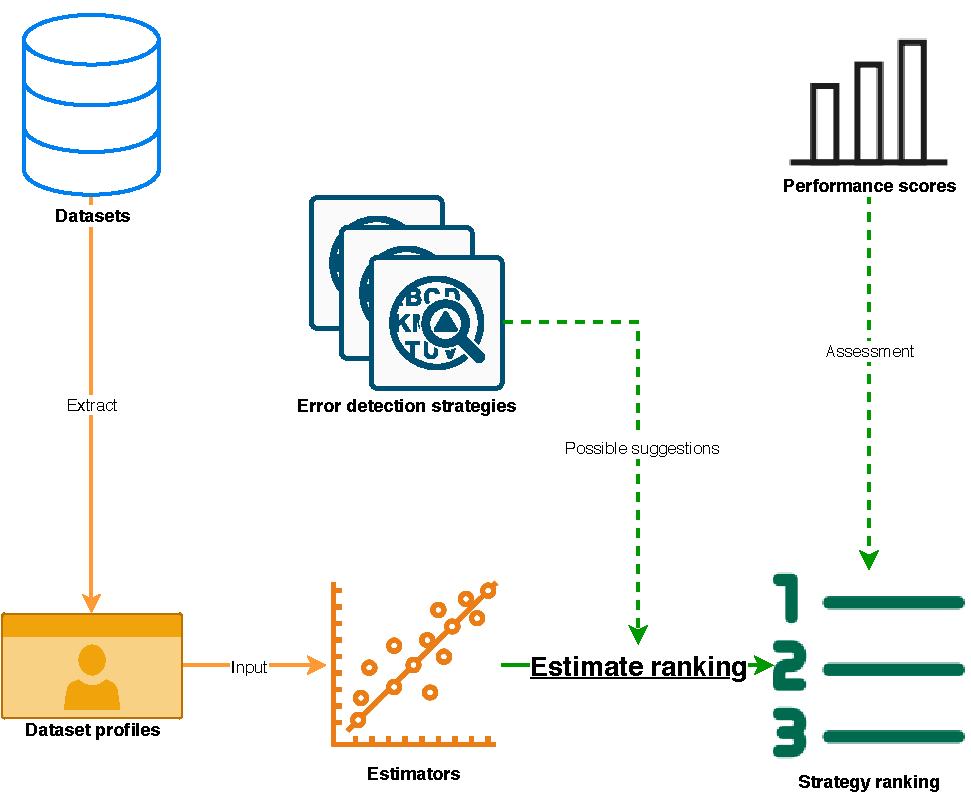
\includegraphics[width=0.9\textwidth]{thesis/Figures/Method/PerformanceEstimation-Ranking.pdf}
    \caption{Flow of the estimation of strategy ranking}
    \label{fig:method_ranking}
\end{figure}

\subsection{Method of ranking}
A user should be able to retrieve an estimated ranking of high performing strategies without running these tools on an unseen dataset. A ranking should be $K$ strategies long, with a predefined $K$. It should be so that a user can a variety of tools and configurations to pick from. To evaluate whether it is possible to create such an estimated ranking, two types of rankings will be made and scored. First, a ranking based on finding the \textbf{best tool} for the dataset will be created. Then, a ranking based on finding the \textbf{best configuration for a tool} will be created.
To test if estimated strategy ranking is viable, this section will focus on F1 estimation and ranking. 
\\To generate an estimated ranking for a new unseen dataset, the data profile as described in \autoref{subsec:dataprofiles} is created. Then, all estimators as found by \autoref{subsec:estimatorselection} are given this data profile as input, generating estimated scores for all strategies $s \in S$. These estimated scores (like a single column in \autoref{tab:estimatedscores}) are then sorted. Depending on the task (best tool or best configuration), the results are filtered and only the top suggestions are kept.

\paragraph{Best tool} First, the ranking of the best tool for a dataset will be discussed. This is the use case where a user does not know which tool he or she wants to use. The tools will be ranked according to the estimated performance score, with one output row per tool. An example of such a ranking is shown in \autoref{tab:ranking_best_tool}. In this example, there are six error detection tools available, just like the six tools used in this research. In the "Tool" column, it is shown which tool is suggested at that ranking. Also, in this ranking, the estimated best configuration for that tool will be suggested in the "Configuration". Lastly, the predicted F1 score will be shown for comparison of predicted performances of the strategies. A user will be able to choose an error detection strategy directly from this list.

\begin{table}[h]
\centering
\begin{tabular}{|l|l|l|l|}
\hline
\textbf{Rank} & \textbf{Tool} & \textbf{Configuration} & \textbf{Estimated F1} \\ \hline
1             & Tool 1        & Config 1-a             & $\hat{y}(s_{1-a}, d)$ \\ \hline
2             & Tool 2        & Config 2-a             & $\hat{y}(s_{2-a}, d)$ \\ \hline
3             & Tool 3        & Config 3-a             & $\hat{y}(s_{3-a}, d)$ \\ \hline
4             & Tool 4        & Config 4-a             & $\hat{y}(s_{4-a}, d)$ \\ \hline
5             & Tool 5        & Config 5-a             & $\hat{y}(s_{5-a}, d)$ \\ \hline
6             & Tool 6        & Config 6-a             & $\hat{y}(s_{6-a}, d)$ \\ \hline
\end{tabular}
\caption{Strategy ranking for best tool}
\label{tab:ranking_best_tool}
\end{table}

\paragraph{Best configuration per tool} Another ranking that could be made is a configuration ranking per tool, for a specific dataset. An example of this ranking is shown in \autoref{tab:ranking_best_configuration}. It might happen that a user has decided to work with a specific tool. However, the user is not aware of the best configuration for that tool. So, for one single tool, $K$ different configurations will be outputted in a ranking. The format of the ranking will be the same as the "best tool" ranking, but only 1 tool type will be shown. As shown in the \autoref{tab:ranking_best_configuration}, in column "Tool", only 1 tool is selected. Then, in the column "Configuration", the different configurations will be ordered from best to worst. Again, the predicted performance score will be displayed in the last column in descending order. 

\begin{table}[h]
\centering
\begin{tabular}{|l|l|l|l|}
\hline
\textbf{Rank} & \textbf{Tool} & \textbf{Configuration} & \textbf{Estimated F1} \\ \hline
1             & Tool 1        & Config 1-a             & $\hat{y}(s_{1-a}, d)$ \\ \hline
2             & Tool 1        & Config 1-b             & $\hat{y}(s_{1-b}, d)$ \\ \hline
3             & Tool 1        & Config 1-c             & $\hat{y}(s_{1-c}, d)$ \\ \hline
4             & Tool 1        & Config 1-d             & $\hat{y}(s_{1-d}, d)$ \\ \hline
5             & Tool 1        & Config 1-e             & $\hat{y}(s_{1-e}, d)$ \\ \hline
6             & Tool 1        & Config 1-f             & $\hat{y}(s_{1-f}, d)$ \\ \hline
7             & Tool 1        & Config 1-g             & $\hat{y}(s_{1-g}, d)$ \\ \hline
8             & Tool 1        & Config 1-h             & $\hat{y}(s_{1-h}, d)$ \\ \hline
9             & Tool 1        & Config 1-i             & $\hat{y}(s_{1-i}, d)$ \\ \hline
10            & Tool 1        & Config 1-j             & $\hat{y}(s_{1-j}, d)$ \\ \hline
\end{tabular}
\caption{Strategy ranking for best configuration per tool}
\label{tab:ranking_best_configuration}
\end{table}

\subsection{Performance measure of ranking}
% To analyze the results of the produced rankings, the ranked strategies of first will be qualitatively be addressed. Generating actual lists of suggested error detection strategies to use and glancing over them will give a first indicates on whether the results will be promising.
Quantitative metrics will be calculated to compare and analyze the results of these rankings.
Average Precision is a metric that takes into account the ranking of the returned documents. Unfortunately, this metric uses a binary relevance scoring, where the last relevant document is equally important to rank high as the first relevant document. In this research, a cutoff point for a score should then be chosen to evaluate, for example, any strategy with a score > 0.5 would be considered relevant. Taking the mean average precision for all different unseen datasets and the produced rankings would then have some meaning, but does not fit this purpose best.

~\\A metric that does take the relative importance into account is the discounted cumulative gain (DCG). It allows degrees of relevance, which is suited for our purpose. The top ranks count the most, meaning whenever a highly relevant (high scoring strategy) is actually listed at the top, the DCG reflects that in a positive way. The utility also decreases with the rank, meaning that lower ranks count less towards the DCG. The DCG is a summation of the relevance score discounted by a log value relative to the given place in the ranking (shown in \autoref{eq:DCG}).
~\\Also, a normalized version of the discounted cumulative gain exists. It takes the ideal ranking and calculates the DCG ($IDCG_k$). The output metric will be the $DCG_k$ for the produced ranking, divided by the DCG for the best ranking (see \autoref{eq:NDCG}). 

\begin{equation}
\label{eq:DCG}
    DCG_k = \sum^k_{r=1} \frac{rel_r}{\log(r+1)}
\end{equation}

\begin{equation}
\label{eq:NDCG}
    NDCG_k = \frac{DCG_k}{IDCG_k}
\end{equation}

The relevance of a returned item in a ranking must be determined beforehand. It should have a relation to how good a strategy performs. 
That is why, for this research, the actual real score (precision, recall or F1) of a strategy run on a specific dataset will be the relevance. This allows this for automatic relevance scoring. As shown in \autoref{fig:method_ranking} and as described in the previous sections, it is possible to assess the produced strategy ranking by using real performance scores from the empirical study as relevance.


\paragraph{Best tool ranking scoring} The best tool ranking will be scored in two ways. When a ranking like displayed in \autoref{tab:ranking_best_tool} is given, scoring can be done tool-wise, but also strategy-wise. The first way is to get the highest relevance for all the configurations of that tool and using that value as $rel_r$. This will judge a ranking solely on the order of tools given. The second way of ranking will be taking the relevance of the suggested strategy for scoring. This is a more difficult task for the recommendation system, as not only does the tool suggestion need to be correct, but the only configuration for that tool should also be the best configuration. 

\subsection{Evaluation}
Again, similarly to \autoref{sec:performanceprediction}, the experiments as proposed above will be assessed qualitatively and quantitatively to answer the third research question: \textit{Is it possible to generate a ranking of tools according to their performance on unseen datasets?}; 

~\\In total, three types of experiments will be conducted. 
\begin{itemize}
    \item Best tool ranking - Scored on tool + configuration relevance
    \item Best tool ranking - Scored on tool relevance
    \item Best configuration ranking - Scored on configuration relevance
\end{itemize}

The estimated rankings will be produced using leave-one-out cross-validation, like in \autoref{sec:performanceprediction}. 

For the first two types of experiments, the same rankings are used. These rankings will consist of 6 entries ($K = 6$), namely for the six possible tools to be suggested. 
For the last type of experiments, the rankings will consist of 10 suggestions\footnote{For this research, a $K$ of 10 will be used. 10 is the number of search suggestions in the basic Google search bar (\url{https://www.google.com/}).} ($K = 10$) of configurations for a tool. Therefore, only tools with 10+ configurations will be tested in this experiment (dBoost \& Raha), as this will test the capability of the ranking system to produce the right order of ranking, but also cutting off the majority of configurations.

For each dataset, the ranking will be scored with NDCG, using the best possible ranking from the ground truth as a reference ideal DCG score. This will result in a NDCG for all datasets available. These scores will the main subject of analysis for evaluation.

\paragraph{Qualitative} The NDCG values per dataset for each experiment will be sorted and plotted for comparison. The focus of the qualitative analysis will be that of the ordering and general relative results between datasets in one experiment. Preferably, NDCG values per dataset are similarly high, without many lower outliers. If there is a cluster of lower NDCG values, the ranking will be deemed meaningless.

\paragraph{Quantitative} Similar to \autoref{sec:performanceprediction}, the results of the experiments will be compared to a baseline method. This baseline method estimates performance as described in \autoref{subsec:evaluation_performanceprediction}. From these baseline estimations, rankings of the same structure as in the experiments will be created and scored with NDCG. While the focus lies on the F1-score for this section, a comparison of mean NDCG for all datasets will be compared for precision-based ranking, recall-based ranking and F1-based ranking, both directly estimated and combinedly estimated (recall + precision estimation to calculate the estimated F1).

The main comparison to answer if it is possible to generate a ranking of tools according to their performance on unseen datasets, will be to see if there is an increase in the mean NDCG for all experiments from the proposed estimator compared to the baseline, described in the paragraph above. If there is no increase in NDCG, the estimator will be deemed not suitable for estimated strategy ranking. 
% RQ4
\section{Interpretability of tools}
\label{sec:interpretabilityoftools}
The prediction of performance of error detection tools gives another research direction, namely the dissection of this prediction.
Based on section \ref{sec:performanceprediction} and \ref{sec:toolranking}, with a set of input features and output values in the two tasks, the regression models can be analyzed to "explain" the inner workings of tools. Using feature importance identification methods depending on the specific regressor or general importance methods, the "weight" of a certain feature can be translated to the performance of a certain tool with a specific configuration. The importance of features for each strategy can than be analyzed, to see if they correspond with the underlying techniques in these methods. If there are matches and mismatches, try to find why the misalignment occurs and see if improvements can be suggested for the error detection tools.

% Introduction of how I feel like implementing this
% Visualizing the Feature Importance for Black Box Models. 

% Black box model

\subsubsection{Feature selection}

\subsubsection{Feature importance}